\documentclass[xcolor=pdftex,dvipsnames,table,mathserif,aspectratio=169]{beamer}
\usetheme{metropolis}
%\usetheme{Darmstadt}
%\usepackage{times}
%\usefonttheme{structurebold}

\usepackage[english]{babel}
%\usepackage[table]{xcolor}
\usepackage{pgf,pgfarrows,pgfnodes,pgfautomata,pgfheaps}
\usepackage{amsmath,amssymb,setspace}
\usepackage[latin1]{inputenc}
\usepackage[T1]{fontenc}
\usepackage{relsize}
\usepackage[absolute,overlay]{textpos} 
\newenvironment{reference}[2]{% 
  \begin{textblock*}{\textwidth}(#1,#2) 
      \footnotesize\it\bgroup\color{red!50!black}}{\egroup\end{textblock*}} 

\DeclareMathSizes{10}{10}{6}{6} 


\title{Bonus Lecture: Numerical Integration}
\author{C.Conlon}
\date{Fall 2020}
\setbeamerfont{equation}{size=\tiny}
\begin{document}

\frame{\titlepage}

\begin{frame}{Numerical Integration}
\begin{itemize}
\item  We are interested in lots of problems that require computing difficult integrals (e.g.: evaluating expectations ).\\
\item Often the problem looks like this:
\begin{align*}
I &= \int_{a}^b h(x) d\,x\\
E_{f| \theta}[g(x)] &= \int_{a}^b g(x) f(x | \theta) d\,x\\
\end{align*}
\item Either just integrating $h(x)$ from $[a,b]$ or computing the expectation of $g(x)$ over some density $f(x)$.
\end{itemize}
\end{frame}


\begin{frame}{Integration Rules}

\begin{itemize}
\item Our goal is to construct an \alert{integration rule} to approximate the function:
\begin{align*}
\int_{a}^{b} f(x) d\, x \approx \sum_{s=1}^S w_s \cdot f(x_s)
\end{align*}
\item Rules consist of \alert{nodes} $x_s$ and \alert{weights} $w_s$
\item This is probably how you learned integration in high school.
\end{itemize}
\end{frame}


\begin{frame}{The Midpoint Rule}
\begin{figure}[htbp]
\begin{center}
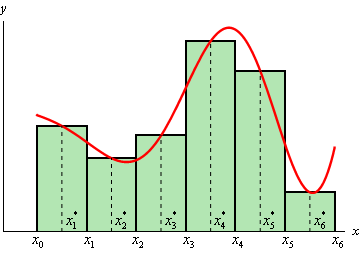
\includegraphics[height=0.65\textheight]{./resources/midpoint.png}
\end{center}
\end{figure}
$$ I = \frac{b-a}{S} \cdot \sum_{s=1}^S f(x_s^{*}) \quad \text{ with }  x_s^{*} = \frac{x_{s+1} + x_{s}}{2}$$
We are fitting \alert{piecewise constants} and adding up \alert{rectangles}
\end{frame}




\begin{frame}{The Trapezoid Rule}
\begin{figure}[htbp]
\begin{center}
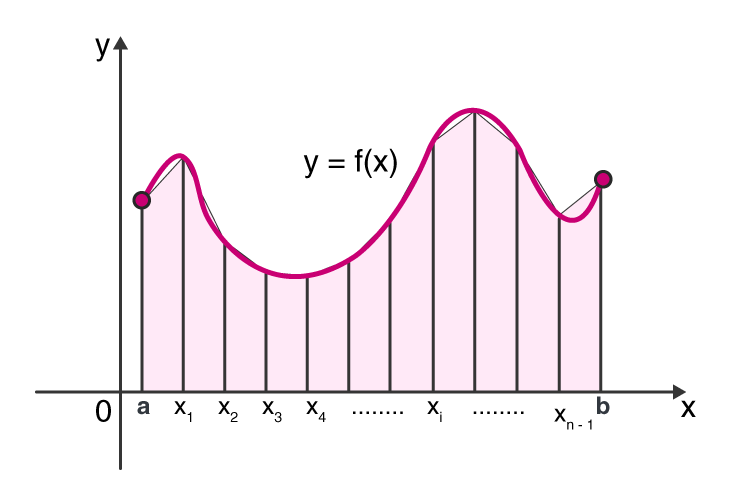
\includegraphics[height=0.65\textheight]{./resources/trapezoid.png}
\end{center}
\end{figure}
$$ I = \frac{b-a}{2 S} \cdot \left[f(x_0) + 2\cdot(f(x_1)+,\ldots,f(x_{S-1})) +  f(x_S) \right] $$
(1) Fit a (piecewise) line from $f(x_s),f(x_{s+1})$; (2) Evaluate trapezoid area analytically; (3) Add up trapezoids.
\end{frame}

\begin{frame}{Simpson's Rule}
\begin{figure}[htbp]
\begin{center}
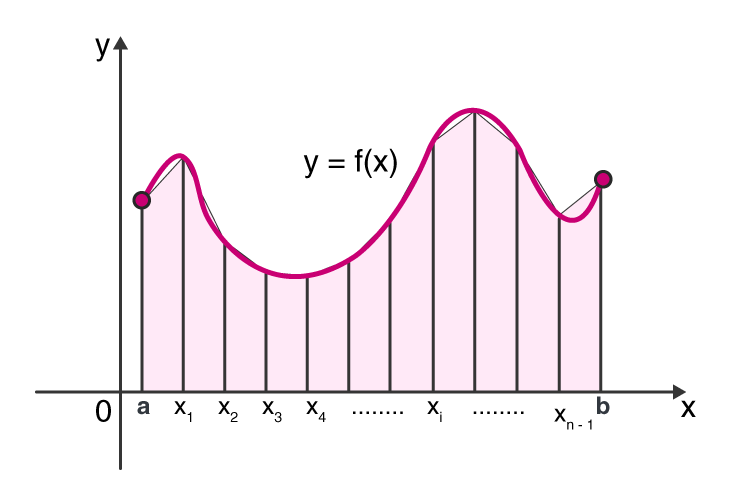
\includegraphics[height=0.65\textheight]{./resources/trapezoid.png}
\end{center}
\end{figure}
$$ I = \frac{b-a}{3S} \cdot \left[f(x_0) + 4(f(x_1)+ f(x_3) +\ldots) + 2(f(x_2)+ f(x_4)+\ldots )  +  f(x_S) \right] $$
(1) Fit a (piecewise) quadratic through $f(x_s),f(x_{s+1}),f(x_{s+2})$; (2) Analytically integrate the quadratic; (3) Add up areas.
\end{frame}


\begin{frame}{Choosing Integration Rules}
Not a lot to choose here
\begin{itemize}
\item Choose the number of points $S$ or interval width $h = \frac{b-a}{S}$.
\item Points are generally equally spaced
\end{itemize}
How accurate is it?
\begin{itemize}
\item \alert{Bounds analysis} is possible (based on series approximations)
\item For Simpson's Rule:
\begin{align*}
\frac{h^{4}}{180}(b-a) \max _{\xi \in[a, b]}\left|f^{(4)}(\xi)\right|
\end{align*}
\item Quadratic approximation does poorly where $f^{(4)}$ is large \\
(and gets up to order 3 polynomials exact).
\end{itemize}
\end{frame}

\begin{frame}{Newton-Cotes Formulas}
Summary of formulas for a single interval:
\begin{center}
\footnotesize
\begin{tabular}{c|c|c|c|c} 
Degree $n$ & Step size $h$ & Common name & Formula & Error term \\
\hline 1 & $b-a$ & Trapezoid rule & $\frac{h}{2}\left(f_{0}+f_{1}\right)$ & $-\frac{1}{12} h^{3} f^{(2)}(\xi)$ \\
\hline 2 & $\frac{b-a}{2}$ & Simpson's rule & $\frac{h}{3}\left(f_{0}+4 f_{1}+f_{2}\right)$ & $-\frac{1}{90} h^{5} f^{(4)}(\xi)$ \\
\hline 3 & $\frac{b-a}{3}$ & Simpson's 3/8 rule & $\frac{3 h}{8}\left(f_{0}+3 f_{1}+3 f_{2}+f_{3}\right)$ & $-\frac{3}{80} h^{5} f^{(4)}(\xi)$ \\
\hline 4 & $\frac{b-a}{4}$ & Boole's rule & $\frac{2 h}{45}\left(7 f_{0}+32 f_{1}+12 f_{2}+32 f_{3}+7 f_{4}\right)$ & $-\frac{8}{945} h^{7} f^{(6)}(\xi)$
\end{tabular}
\url{https://en.wikipedia.org/wiki/Newton-Cotes_formulas}
\end{center}
\end{frame}


\begin{frame}{Can we do better?}
Can use \alert{adaptive rules} (built-in many software routines)
\begin{itemize}
\item Divide up $[a,b]$ evenly into sub-intervals
\item Some are relatively flat or well-approximated, some are not.
\item Use more points in the sub-intervals that are the most difficult to approximate
\item Don't waste points in intervals that are easy to approximate.
\end{itemize}
Drawbacks
\begin{itemize}
\item Points used in approximation are $f(\cdot)$ dependent
\item Points used in approximation $x_s$ may not be the same for $f(x | \theta)$ at all values of parameters $\theta$.
\end{itemize}
\end{frame}



\begin{frame}{Gaussian Quadrature: Same Basic Idea}
\begin{itemize}
\item Choose a degree of polynomial approximation for $f(x)$ on $[a,b]$.
\item ``Fit'' the polynomial by evaluating $f(x_s)$ at various values of $x_s$
\item Integrate the polynomial analytically by adjusting coefficients on $f(x_s)$.
\end{itemize}
In practice, much easier: get a pre-specified set of weights and nodes $(w_s,x_s)$.
\end{frame}

\begin{frame}{Gaussian Quadrature: But a little different}

\begin{itemize}
\item $[1,x,x^2,x^3,\ldots]$ is not the only \alert{polynomial basis}.
\item For example \alert{Chebyshev Basis} (of first kind) is \alert{orthogonal} $[1,x,2x^2-1,4x^3-3x,\ldots]$
\item Concept remains the same:
\begin{enumerate}
\item Approximate $f(x)$ with a polynomial basis
\item Integrate the polynomial exactly
\item In practice we just get a pre-determined set of points and weights $(x_s,w_s)$ for a given polynomial order.
\end{enumerate}
\item Rules have some additional properties
\begin{itemize}
\item What interval to integrate over $[-1,1]$ or $[0,\infty)$ or $(-\infty,+\infty)$.
\item Can we exploit properties of $f(x)$: is it proportional to $\frac{1}{\sqrt{1-x^2}}$ or $e^{-x}$ or $e^{-x^2}$?
\end{itemize}
\item May need to do change of variables on $f(x) \rightarrow f(v)$ to better satisfy conditions above.
\end{itemize}
\end{frame}


\begin{frame}{Gaussian Quadrature}
\small
Formulas look like:
\begin{eqnarray*}
\int_{a}^b f(x) d x \approx \sum_{s=1}^S  w_s f(x_s)
\end{eqnarray*}
for some quadrature nodes $x_s \in [a,b]$ and weights $w_s$.
\begin{itemize}
\item Let $\mathcal{F}_k$ be the space of degree $k$ polynomials
\item Quadrature formulas are exact of degree $k$ if it correctly integrates each function in $\mathcal{F}_k$
\item Gaussian quadrature formulas use $S$ points and are exact of degree $2s-1$.
\end{itemize}
Approximation Error
\begin{eqnarray*}
\int_a^b w(x) f(x)  dx - \sum_{s=1}^S w_s f(x_s) = \frac{f^{(2S)}(\xi)}{(2S)!} (p_S,p_S) 
\end{eqnarray*}
\end{frame}


\begin{frame}{Gaussian Quadrature}
\begin{description}
\item[Legendre] Domain: $[-1,1]$, $w(x) = 1$
\item[Chebyshev] Domain: $[-1,1]$, $w(x) = \frac{1}{\sqrt{1-x^2}}$
\item[Laguerre] Domain: $[0,\infty)$, $w(x) = \exp[-x]$ (useful for present value)
\item[Hermite] Domain: $(-\infty,\infty)$, $w(x) = \exp[-x^2]$ (useful for normal)
\end{description}
Helpful if function is $C^{\infty}$ or real-analytic (comports with series expansion).
\end{frame}



\begin{frame}{Alternative: Monte Carlo Integration}
\begin{align*}
E_{f| \theta}[g(x)] &= \int_{a}^b g(x) f(x | \theta) d\,x\\
&\approx \frac{1}{S} \sum_{s=1}^S g(x_s)
\end{align*}
\begin{itemize}
\item Sample $[x_1,\ldots,x_S]$ by drawing from $f(x | \theta)$.
\item Weight everything equally $\frac{1}{S}$
\item Can't bound errors, but can discuss rate of convergence
\item Convergence is slow $\frac{1}{\sqrt{S}}$ but mostly unrelated to curvature of $f(\cdot)$.
\end{itemize}
\end{frame}


\begin{frame}{Monte Carlo Integration: Change of Variables}
Still often want to change variables. Consider $f(x | \theta) \sim N(\mu,\sigma^2)$
\begin{itemize}
\item Should we sample from $x_s \sim N(\mu,\sigma)$?
\item Might be better to sample $z_s \sim N(0,1)$ and then $x_s = z_s\cdot \sigma + \mu$
\item For complicated distributions $v_s \sim U[0,1]$ and then $x_s = \Phi^{-1}(v_s) \cdot \sigma + \mu$
\end{itemize}
Discuss approximating $\pi$.
\end{frame}

\begin{frame}{Example: Gauss Herrmite}
Let $Y\sim N(\mu,\sigma^2)$ and apply COV $x = (y-\mu)/\sqrt{2} \sigma$
\begin{eqnarray*}
E[f(Y)] = (2 \pi \sigma^2)^{-\frac{1}{2}} \int_{-\infty}^{\infty} f(y) \exp\left[-\frac{(y-\mu)^2}{2\sigma^2} \right] dy \\
\int_{-\infty}^{\infty} f(y) \exp\left[-\frac{(y-\mu)^2}{2\sigma^2} \right] dy = \int_{-\infty}^{\infty} f(\sqrt{2} \sigma x + \mu) e^{-x^2} \sqrt{2} \sigma dx
\end{eqnarray*}
Gives the quadrature formula using Gauss Hermite $(x_s,w_s)$.
\begin{eqnarray*}
E[f(Y)] = \frac{1}{\sqrt{\pi}} \sum_{s=1}^S w_s f(\sqrt{2}\sigma x_s+ \mu)
\end{eqnarray*}
notice that we don't have the $e^{-x^2}$ anymore.
\end{frame}



\begin{frame}{Quasi Monte Carlo}
Lots of ways to improve on purely pseudorandom sampling
\begin{itemize}
\item Antithetic draws
\item Low-discrepancy sequence (Halton, Sobol, Low-discrepancy sequence etc.) 
\item Think about these as ensuring more even coverage (stratified).
\item Koksma-Hlawka inequality gives bounds but is hard to characterize the Hardy-Kruse variation of $f(\cdot)$.
\end{itemize}
Many of these are built-in routines in Python, R, Matlab, etc.
\end{frame}







\begin{frame}{Higher Dimensional Integration}
\begin{itemize}
\item In higher dimension we can use product rules of 1-D integrals. $\mathbf{x_s^{(1)}} \times \mathbf{x_s^{(2)}}$ and $\mathbf{w_s^{(1)}} \times \mathbf{w_s^{(2)}}$
\item This grows exponentially in dimension $D$ (Curse of Dimensionality)
\begin{itemize}
\item 10 points in dimension one, means 10{,}000 points in dimension 4.
\end{itemize}

\item Monte Carlo is not cused but slow to converge $\frac{1}{\sqrt{S}}$ vs $\frac{1}{2S!} f^{(2S)}$
\item Some monomial rules (Judd), (Skrainka and Judd) aren't cursed
\item Sparse Grids show how to combine 1-D rules more efficiently (\url{www.sparse-grids.de})
\end{itemize}
\end{frame}



\end{document}